\section{Interpretation and Limits}
\label{sec:discussion}

\subsection{Response Fit, Severity and Source Identity}
\label{sec:narrative-information}

A retained physical history predicts the response still present after
restoration and defines the state from which a new intervention begins.
For the exact observation map $\Psi$ and the same pre-intervention history
$h$, the incremental response is
\begin{equation}
 s_{e\mid h}(t)=\Psi_t(h\oplus e)-\Psi_t(h).
 \label{eq:history-increment}
\end{equation}
The two paths share their initial physical and instrumental states.
In an additive linear time-invariant system, superposition makes this
increment independent of the prior state. Nonlinear dynamics can change
its shape, but do not guarantee greater source separation. Preserving
recovery is a model-consistency requirement, not a claim that an earlier
disturbance universally helps localization. The stream implementation
approximates these paths with its declared switched predictors; it does
not solve the full nonlinear DAE for each hypothesis.

A better physical prediction need not produce a better location. Competing
sources may remain similar after their severities and initial conditions
are fitted. For a response $s_h$ at specified severity and context, the
distance to an admitted competitor is
\begin{equation}
 d_h^2=\min_{j\ne h}\ \min_{\beta_j\in\mathcal A_j}
       \|s_h-s_j(\beta_j)\|_{\Sigma^{-1}}^2.
 \label{eq:narrative-separation}
\end{equation}
The set $\mathcal A_j$ fixes allowed signs, severities and nuisance
coordinates. Small distance makes source discrimination noise-sensitive;
it is not a universal error formula or a calibrated decision certificate
\cite{eriksson2013diagnosability,scharf1994matched}.

Three outcomes remain separate: prediction error at a specified physical
source, ranking of competing sources, and uncertainty calibration. A
response improvement establishes the first. It establishes the second only
if source decisions improve under the same observations, horizon and
decision rule. Neither establishes the third automatically. A nonlinear
response comparison is needed before treating a surrogate's residual
confusion as an unavoidable physical limit.

The supplementary archive retains the earlier state-reconstruction and
simultaneous-load studies, with their separate observation contracts and
prior-normalization qualification. Their known-onset scores are not
combined with the causal results here. In particular, recovering hidden
voltages does not certify the source that moved them.

To first order, a component of the context derivative parallel to a nominal
source signature can be absorbed by fitting a different severity. Correct
source ranking can therefore coexist with biased intensity. Components
orthogonal to that signature cannot be removed by this rescaling. This
explains why source accuracy can reach a test ceiling while response and
severity errors still distinguish the models; it is a standard projection
argument, not a new identifiability theorem.


\subsection{Does Recovery Increase Source Separation?}
\label{sec:recovery-control}

A separate physical control tests this possibility without changing the
stream method. We solve 38 complete F01 trajectories of 8 s with 241 PMU
reports each. A prior 8\% load change at bus 7 or 24 is applied at 2 s and
restored at 3 s. A weak 0.06\% load change follows after 0.5 or 2 s.
The candidate pairs are 18/27, 16/21 and 3/21, and the observation horizon
is 1.5 s. Controls and prior-severity differences account for the remaining
trajectories. Within each matched history, the secondary-event and
no-secondary-event trajectories share the same prefix. Physical and
instrumental states are retained through restoration.

This is an oracle component test: the prior trajectory, secondary onset,
load family and candidate pair are supplied. Finite-amplitude differences
of nonlinear trajectories provide incremental responses; these are
secants, not newly derived analytical tangents. The 47-coordinate F01
measurement operator is followed by its frozen innovations transform.
For a geometric control, we profile nonnegative competing amplitudes.
Adding a rank-one covariance from uncertainty of 0.01 in the previous load
fraction tests sensitivity to a nuisance direction; it is not a causal
posterior over the full state.

\begin{figure*}[t]\centering
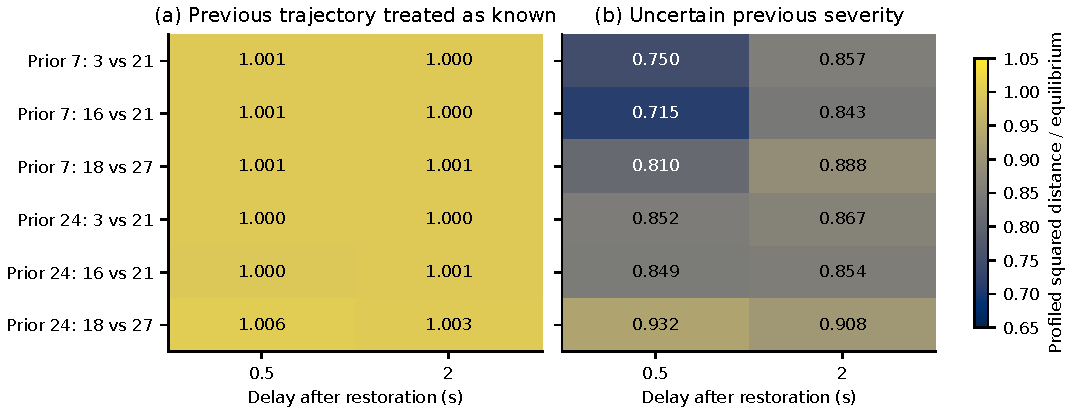
\includegraphics[width=0.98\textwidth]{figures/generated/recovery_x04_information.pdf}
\caption{Full-F01 physical control, not an R11 performance comparison.
Each cell is the profiled squared separation during recovery divided by
its equilibrium value. The same source pairs are evaluated with the
previous trajectory treated as known (left) and with one uncertain
previous-severity direction (right). Values below one mean less separation.
Adding nuisance covariance reduces precision at fixed signatures by
construction; the left panel separately shows the small change in
physical response geometry. The 12 cells share four recovery histories.}
\label{fig:recovery-x04}\end{figure*}

The median ratio is 1.0006 with known history and 0.8532 with that nuisance
direction; none of the 12 latter ratios exceeds one
(Fig.~\ref{fig:recovery-x04}). An illustrative binary likelihood comparison,
using a signed Gaussian amplitude prior of standard deviation 0.0015 and
300 common Gaussian innovation draws per generating source, gives the
same mean accuracy, 98.35\%, for equilibrium and conditioned signatures.
Two cells worsen and one improves. This likelihood experiment integrates
signed amplitudes, whereas the distance profiles nonnegative amplitudes;
the distance is not asserted to bound its error. The noise assumption is
an innovations-domain control, not validation of the complete instrumental
generator. These correlated, known-onset comparisons establish neither
an R11 improvement nor general equivalence. They provide no support for
claiming that recovery universally creates useful source information.


\subsection{Operational Meaning and Scope}
The physical distinction underlying the stream method is simple:
restoration changes an input or topology, but does not erase the machine
state. Retaining that state lets recovery compete with a new intervention.
The development comparison also shows why alarm count and timely location
must be reported together. Stricter admission can suppress extras while
rejecting a real load. The existing admission ablation does not isolate
the contribution of every recovery-memory operation.

\IfFileExists{generated/ei_x02_macros.tex}{The signature experiment addresses
a different source of error. Its corrected variants receive the same
pre-event measurements and offset. Any difference between them therefore
comes from the event--context term and its estimated context, rather than
a privileged baseline or longer window. This isolates the tested response
approximation, but not an improvement of the unchanged causal detector.
Known timing, one scalar context and four load sources make it a controlled
component test.}{Changing an operating reference can also leave the event
response misspecified. A matched signature experiment is needed to
distinguish that error from an onset or recovery failure.}

Our construction builds on trajectory-based diagnosis, sequential
likelihoods and multiple-model filtering. Their general principles are not
new contributions here. The methodological claim concerns the specified
competition among intervention and recovery histories; the experiments
measure its operational behavior. Numerical superiority is claimed only
where a common-data comparison supports it, not over Warner or other
procedures that were not executed.

The continuous catalog contains nine load buses and nine lines and requires
an intervention-free startup. Missing PMUs, unknown families, source-excluded
causal transfer and field operation are untested. F01 retains a provisional
BUS5 current terminal and excludes BUS39 current angle. Agreement with
this research model does not establish the producer's CT placement or
exact reproduction of RAW0001. Local predictors, history pruning, covariance
approximations and fitted startup parameters also limit probability claims.

F01's noise port applies temporal and cross-PMU structure within each
signal family. Its archived cross-family factor covariance is not applied,
and frequency/ROCOF noise is added after phase estimation. The inference
comparison therefore concerns this declared simulator, not the complete
dependence structure of a physical PMU installation.

The two ExtraTrees adapters are particular frozen implementations. Their
load-transfer failure does not rule out learned load diagnosis or establish
a better official hackathon score. Chen's eligible test concerns persistent
line openings; its F01 adapter has DC/white-injection assumptions that do
not capture all instrumental effects. Its mismatches and censored decisions
remain part of the comparison.

Joint context uncertainty, unrestricted simultaneous sources and calibrated
posterior probabilities remain unvalidated. Such extensions must preserve
source-discriminating response directions and account for dependence
between estimation error and measurement noise.

Finally, processing reports causally is not proof of real-time throughput.
Observation time, computation and queue delay must be measured separately.
The present implementations remain research inference services rather
than validated protection or control systems.
